\section{Datenbankzugriff}\label{sec:datenbankzugriff}
Die zentrale Komponente unseres Systems ist die Datenbank. In sie fügt der Crawler neue Datensätze ein und aktualisiert Vorhandene. Der Kategorisierer ist dafür zuständig, dass die gefundenen Accounts nach der DMOZ.org Datenbank in Kategorien unterteilt werden. Die GUI wiederum ist die Komponente die die Daten aus der Datenbank ausliest und visualisiert. Gegebenenfalls kann sie auch Einträge verändern beziehungsweise vervollständigen.
\\Da alle unsere drei Systemkomponenten lesend, sowie schreibend auf die Datenbank zugreifen, haben wir uns entschlossen ein Paket für den Datenbankzugriff für alle Komponenten zur Verfügung stellen. Dieses sogenannte mysql-Package ist dann für den Auf- und Abbau der Verbindung zur Datenbank zuständig, sowie für das Schreiben und Lesen in beziehungsweise aus der Datenbank. Es stellt für jede der drei Komponenten ein eigenes Interface zur Verfügung, sodass jede Komponente nur die für sie erlaubten Änderungen an der Datenbank vornehmen kann.
In \cref{fig:mysql-package} ist der Aufbau des mysql-Packages zu sehen. Das darin eingeschlossene result-Package stellt Objekt und Methoden zu Verfügung um die Ergebnisse aus der Datenbank zu speichern und zu verarbeiten.

\begin{figure}[h!]
	\centering
	\includegraphics[width=\textwidth,height=\textheight,keepaspectratio=true]{dia/uml_mysql-package}
	\caption{UML-Klassendiagramm des mysql-Packages}
	\label{fig:mysql-package}
\end{figure}

\begin{description}
	\item[AccessData] Klasse zur Verwaltung von Zugriffsdaten für die Datenbank.
	\item[DBConnection] Abstrakte Klasse die eine Verbindung zu einer Datenbank aufbaut und diese Verbindung auch wieder trennt.
	\item[DBIcrawler] Interface welches die Methoden spezifizieren die der Crawler für den Datenbankzugriff benötigt.
	\item[DBIcategorizer] Interface welches die Methoden spezifizieren die der Kategorisierer für den Datenbankzugriff benötigt.
	\item[DBIgui] Interface welches die Methoden spezifizieren die die GUI für den Datenbankzugriff benötigt.
	\item[DBcrawler] Diese Klasse implementiert die Methoden des DBIcrawler Interfaces und stellt dem Crawler eine Datenbankverbindung zur Verfügung.
	\item[DBcategorizer] Diese Klasse implementiert die Methoden des DBIcategorizer Interfaces und stellt dem Kategorisierer eine Datenbankverbindung zur Verfügung.
	\item[DBgui] Diese Klasse implementiert die Methoden des DBIgui Interfaces und stellt dem Client / der GUI eine Datenbankverbindung zur Verfügung.
	\item[Result] Als abstrakte Klasse stellt Result eine Möglichkeit zum Speichern des Datenbankindexes von Datenbankeinträgen zur Verfügung.
	\item[Account] In dieser Klasse werden einzelne Accounts verwaltet und gespeichert.
	\item[Retweets] In dieser Klasse werden nach Orten (und eventuell nach Daten) gruppierte Retweets verwaltet und gespeichert.
	\item[Tweets] In dieser Klasse werden nach Daten gruppierte Tweets verwaltet und gespeichert.
	\item[Location] In dieser Klasse werden einzelne Orte verwaltet und gespeichert.
	\item[Category] In dieser Klasse werden einzelne Kategorien verwaltet und gespeichert.
\end{description}

\section{ER-Modell}
Die Datenbank besteht aus sieben Tabellen, die über Fremdschlüssel miteinander in Relation stehen (s. \cref{fig:mysql-er}).
\begin{description}
	\item[Accounts] enthält alle verifizierten Accounts, die der Crawler im Twitter Stream mitgelesen hat bzw. die in der GUI hinzugefügt wurden. Dabei entspricht \emph{TwitterAccountId} der ID des Accounts in Twitter und \emph{id} ist ein Datenbank interner Primärschlüssel. Die Attribute \emph{Verified}, \emph{URL} und \emph{AccountName} entsprechen jeweils in Twitter hinterlegten Daten. \emph{Categorized} gibt an ob dieser Account bereits kategorisiert wurde und \emph{LocationId} enthält den vom Loakaliserer berechneten zugehörigen Ort.
	\item[Category] speichert die hierarchisch strukturierten (\emph{ParentId}) Kategorien.
	\item[AccountCategory] stellt die Relation zwischen	\emph{accounts} und \emph{category} in einer separaten Tabelle her, da einem Account mehrere Kategorien zugeordnet werden können.
	\item[Location] enthält die vom Lokalisierer ermittelten Orte, die jeweils \emph{Code} und \emph{Name} enthalten und auch per \emph{ParentId} hierarchisch gegliedert sind.	
	\item[Day] enthält unterschiedliche Daten (\emph{Day}), die mittels \emph{Id} referenziert werden.
	\item[Tweets] beinhaltet die Anzahl der Tweets (\emph{Counter}) eines Accounts (\emph{AccountId}) bis zu einem bestimmten Tag (\emph{DayId}).
	\item[Retweets] speichert die Anzahl der Retweets (\emph{Counter}) der Tweets eines Accounts (\emph{AccountId}) bis zu einem bestimmten Tag (\emph{DayID}) innerhalb eines bestimmten Lands bzw. Orts (\emph{LocationId}).
\end{description}
\begin{figure}[h!]
	\centering
	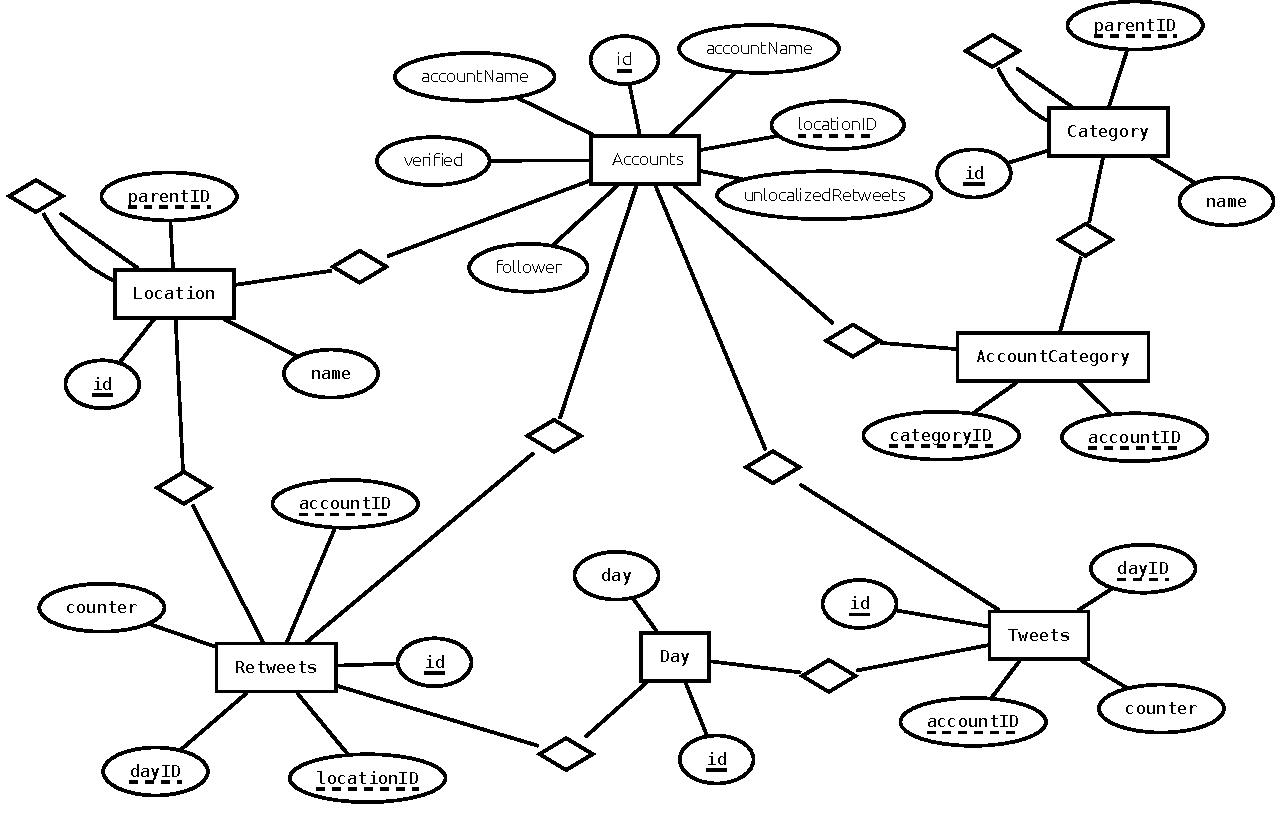
\includegraphics[width=\textwidth,height=\textheight, keepaspectratio=true]{dia/er}
	\caption{ER-Modell der MySQL-Datenbank}
	\label{fig:mysql-er}
\end{figure}
